\documentclass[border=4pt]{standalone}
\usepackage[siunitx]{circuitikz}

\begin{document}
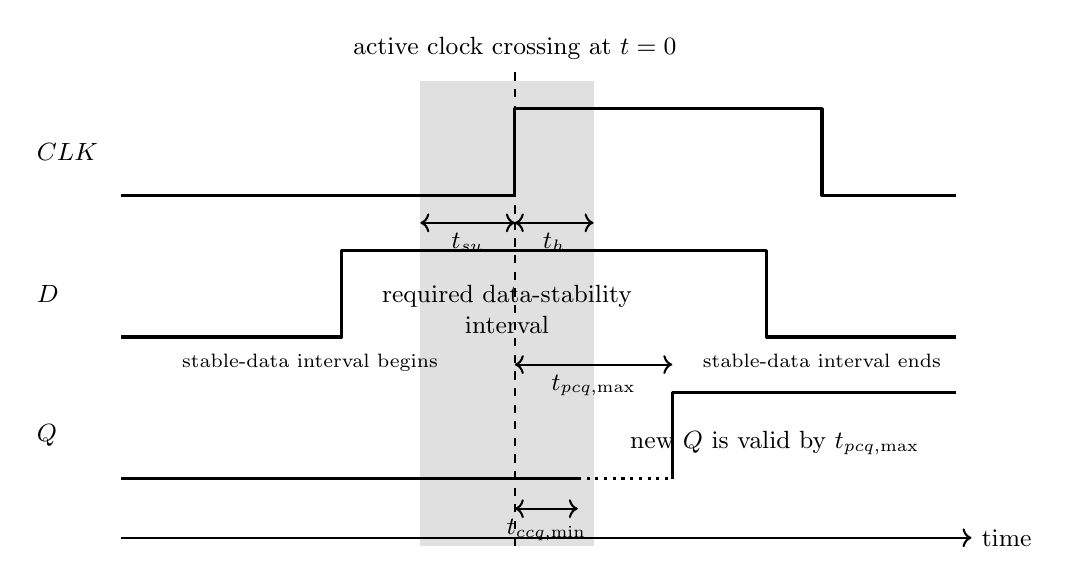
\begin{tikzpicture}[x=1cm,y=1cm,line width=0.75pt,
  thick/.style={line width=1.15pt,line join=round}]
  \definecolor{stability}{gray}{0.88}
  \fill[stability] (5.0,0.25) rectangle (7.2,6.15);
  \draw[dashed] (6.2,0.25) -- (6.2,6.3);
  \node[font=\small, above] at (6.2,6.3) {active clock crossing at $t=0$};

  \node[font=\small, right] at (0.0,5.25) {$CLK$};
  \node[font=\small, right] at (0.0,3.45) {$D$};
  \node[font=\small, right] at (0.0,1.65) {$Q$};
  \draw[->] (1.2,0.35) -- (12.0,0.35) node[right,font=\small] {time};

  \draw[thick] (1.2,4.7) -- (6.2,4.7) -- (6.2,5.8) -- (10.1,5.8)
    -- (10.1,4.7) -- (11.8,4.7);
  \draw[thick] (1.2,2.9) -- (4.0,2.9) -- (4.0,4.0) -- (9.4,4.0)
    -- (9.4,2.9) -- (11.8,2.9);
  \draw[thick] (1.2,1.1) -- (7.0,1.1);
  \draw[thick,dotted] (7.0,1.1) -- (8.2,1.1);
  \draw[thick] (8.2,1.1) -- (8.2,2.2) -- (11.8,2.2);

  \draw[<->] (5.0,4.35) -- (6.2,4.35)
    node[midway, below,font=\small] {$t_{su}$};
  \draw[<->] (6.2,4.35) -- (7.2,4.35)
    node[midway, below,font=\small] {$t_h$};
  \draw[<->] (6.2,0.72) -- (7.0,0.72)
    node[midway, below,font=\small] {$t_{ccq,\min}$};
  \draw[<->] (6.2,2.55) -- (8.2,2.55)
    node[midway, below,font=\small] {$t_{pcq,\max}$};
  \node[font=\small,align=center] at (6.1,3.25)
    {required data-stability\\interval};
  \node[font=\small, align=center] at (9.5,1.55)
    {new $Q$ is valid by $t_{pcq,\max}$};
  \node[font=\scriptsize, below] at (3.6,2.82) {stable-data interval begins};
  \node[font=\scriptsize, below] at (10.1,2.82) {stable-data interval ends};
\end{tikzpicture}
\end{document}
